% !TEX program = xelatex
\documentclass[a4paper]{article}
\usepackage{amsthm}
\usepackage{amssymb}
\usepackage{bm}
\usepackage{mathtools}
\usepackage[x11names]{xcolor}
\usepackage{xparse}
\usepackage{fontspec}
\usepackage{unicode-math}
\setromanfont{DovesType-Regular.otf}
\setsansfont{Andika}
\setmathfont{Asana Math}[Scale=1]

% \usepackage{pstricks}
\usepackage{varwidth}
\usepackage{siunitx}
\usepackage{graphicx}
\usepackage[margin=1cm]{geometry}
\usepackage[most]{tcolorbox}
\usepackage{pgfplots}
\pgfplotsset{compat=newest}
\tcbuselibrary{skins,xparse,poster,breakable}
% \usetikzlibrary{fadings}
\usetikzlibrary{calc, plotmarks, shapes, shapes.geometric, positioning, angles, intersections, quotes, through, patterns, turtle, arrows.meta}
\usetikzlibrary{decorations.markings,backgrounds}
% \usepackage{etoolbox}
% \usepackage{tkz-euclide}
% \usepackage{xlop}
% \newcommand\hole[2]{#1}  % for use with xlop
\pagenumbering{gobble}
%%%%%%%%%%%%%%%%%%%%%%%%%%%%%%%%%%%%%%%%%%%%%%%%%%%%%%%%%
\newcommand\markangle[9]{% origin X Y radius radiusmark mark colour opacity
%  % fill red circle offset-from-centre
  \begin{scope}
    \path[clip] (#1) -- (#2) -- (#3);
    \fill[color=#7,fill opacity=#8,draw=black,name path global=pcircle]  % global declaration required otherwise pcircle is not seen by the `named intersections=' lines below.
    (#1) circle (#4);
  \end{scope}
  % middle calculation
  \path[name path=line one] (#1) -- (#2);
  \path[name path=line two] (#1) -- (#3);
  \path[%
  name intersections={of=line one and pcircle, by={inter one}},
  name intersections={of=line two and pcircle, by={inter two}}
  ] (inter one) -- (inter two) coordinate[pos=#9] (place);
  % put mark
  \node at ($(#1)!#5!(place)$) {\scriptsize{#6}};
}

\newcommand\tcircle[6]{% centre coord (x,y), radius, points, radpoint, colour, edge
  \coordinate (O) at (#1,#2); % centre of the circle
  \def\radius{#3}          % radius of the circle
  \def\npts{#4}            % number of the points
  \def\radpt{#5}           % radius of the points
  \colorlet{ptcolour}{#6}  % colour of the points
  % \draw (O) circle (\radius);
  \foreach \numpoint in {1,...,\npts}{
    \fill[ptcolour] (O) ++ (360/\npts*\numpoint:\radius) coordinate (C\numpoint) circle(\radpt);
  }
}

% \newcommand{\condSoln}[2]{\ifcsdef{r@#1}{#2}{}}

% \newcommand\fadingtext[3][]{%
%    \begin{tikzfadingfrompicture}[name=fading letter]
%      \node[text=transparent!0,inner xsep=0pt,outer xsep=0pt,#1] {#3};
%    \end{tikzfadingfrompicture}%
%    \begin{tikzpicture}[baseline=(textnode.base)]
%      \node[inner sep=0pt,outer sep=0pt,#1](textnode){\phantom{#3}};
%      \shade[path fading=fading letter,#2,fit fading=false]
%      (textnode.south west) rectangle (textnode.north east);%
%    \end{tikzpicture}%
% }

\definecolor{JISpurple}{RGB}{89,72,122}
\definecolor{JISivory}{RGB}{241,234,221}
\definecolor{JIStaupe}{RGB}{183,156,154}
\definecolor{PaleGreen}{RGB}{240,255,240} % 'Honeydew'

\AddToHook{shipout/background}{%
    \put (0in,-\paperheight){
\includegraphics[width=\paperwidth,height=\paperheight]{images/R10V5-R.png}}%
}

\newcommand\numberthis{\addtocounter{equation}{1}\tag{\theequation}}

\newtcolorbox{MyOuterBox}{%
  enhanced,
  breakable,
  frame style=JISpurple,
  colback=JISivory,
  colframe=JISpurple,
  title={
\includegraphics[width=0.9cm,height=0.9cm]{images/JIS Final Logo FA-02.png}\raisebox{3mm}{\Large{Maths Challenge}\hspace{26em} \Large{\bfseries\sffamily 11}}},
}

\newtcolorbox{MyInnerBox}[2][]{enhanced,%empty,
coltitle=JISpurple,colback=white,
breakable,
fonttitle=\bfseries\sffamily,
attach boxed title to top left={yshift=-1.5mm},
boxed title style={empty, size=small, top=1mm, bottom=0pt},
varwidth boxed title=0.5\linewidth,
frame code={
  \path (title.east|-frame.north) coordinate (aux);
\path[draw=JISpurple, line width=0.5mm, rounded corners,fill=white]
(frame.west) |- ([xshift=-2.5mm]title.north east) to[out=0, in=180] ([xshift=7.5mm]aux)-|(frame.east)|-(frame.south)-|cycle;
},
title={#2},#1}

\newtcolorbox{MyInnerSplitBox}[2][]{enhanced,%empty,
bicolor,sidebyside,sidebyside align=top seam,
righthand width=8.5cm,colbacklower=white,
sidebyside gap=5mm,
breakable,
coltitle=JISpurple,colback=white,
fonttitle=\bfseries\sffamily,
attach boxed title to top left={yshift=-1.5mm},
boxed title style={empty, size=small, top=1mm, bottom=0pt},
varwidth boxed title=0.5\linewidth,
frame code={
  \path (title.east|-frame.north) coordinate (aux);
\path[draw=JISpurple, line width=0.5mm, rounded corners,fill=white]
(frame.west) |- ([xshift=-2.5mm]title.north east) to[out=0, in=180] ([xshift=7.5mm]aux)-|(frame.east)|-(frame.south)-|cycle;
},
title={#2},#1}


\newtcolorbox{MySolutionBox}[1][]{%
  enhanced,
  breakable,
  frame style=JISpurple,
  colback=PaleGreen, colframe=green,
  title={\Large Solution},
  drop fuzzy shadow,
  halign=left,
  #1
}

%%%%%%%%%%%%%%%%%%%%%%%%%%%%%%%%%%%%%%%%%%%%%%%%%%
\newtoggle{SOLUTION}
%%% Uncomment the appropriate line below to show solutions %%%
% \toggletrue{SOLUTION}
\togglefalse{SOLUTION}
%%%%%%%%%%%%%%%%%%%%%%%%%%%%%%%%%%%%%%%%%%%%%%%%%


%%%%%%%%%%%%%%%%%%%%%%%%%%%%%%%%%%%%%%%%%%%%%%%%%%
%%%%%%            DOCUMENT BEGINS           %%%%%%
%%%%%%%%%%%%%%%%%%%%%%%%%%%%%%%%%%%%%%%%%%%%%%%%%%
\begin{document}


  \begin{MyOuterBox}
    \iftoggle{SOLUTION}{Here are the full, or partial solutions.
    }{
      Welcome to this week's Maths Challenge!\\
      It's fine to have a go at both questions!\\
      Solutions must be explained in detail, responses with just the answer may be ignored.\\
      Drop your solution in the box in the staffroom by Tuesday.
    }
       \begin{MyInnerBox}{Year 8 and below}
     \begin{minipage}[b]{0.33\textwidth}
     \begin{tikzpicture}[scale=0.85]
        \tcircle{0}{0}{3}{12}{0.05}{black};
        \filldraw[yellow,fill=yellow] (C8) -- (C3) -- (C4) -- cycle;
        \draw[yellow,fill=yellow] (C3) arc [start angle=90, end angle=120, radius=3] -- cycle;
        \draw[thick, black] (C8) -- (C3) (C8) -- (C4);
        \filldraw[yellow,fill=yellow] (C8) -- (C5) -- (C6) -- cycle;
        \draw[yellow,fill=yellow] (C5) arc [start angle=150, end angle=180, radius=3] -- cycle;
        \draw[thick, black] (C8) -- (C5) (C8) -- (C6);
        \filldraw[yellow,fill=yellow] (C8) -- (C1) -- (C2) -- cycle;
        \draw[yellow,fill=yellow] (C1) arc [start angle=30, end angle=60, radius=3] -- cycle;
        \draw[thick, black] (C8) -- (C1) (C8) -- (C2);
        \filldraw[yellow,fill=yellow] (C8) -- (C11) -- (C12) -- cycle;
        \draw[yellow,fill=yellow] (C11) arc [start angle=-30, end angle=0, radius=3] -- cycle;
        \draw[thick, black] (C8) -- (C11) (C8) -- (C12);
        % \filldraw[yellow,fill=yellow] (C8) -- (C9) -- (C10) -- cycle;
        \draw[yellow,fill=yellow] (C8) arc [start angle=-120, end angle=-60, radius=3] -- cycle;
        \draw[thick, black] (C8) -- (C10);
        \draw (O) circle (\radius);
        \iftoggle{SOLUTION}{
        \draw[-Stealth,blue] (0,-2.78) -- (-2.4,-1.5);
        \draw[-Stealth,blue] (1,-1.5) -- (-2,0);
        \draw[-Stealth,blue] (1.3,1) -- (0,1.7);
        }{}
      \end{tikzpicture}%
    \end{minipage}%
      % \hspace{0.3cm}
     \begin{minipage}[b]{0.33\textwidth}
       \raisebox{-3mm}{
      \begin{tikzpicture}[scale=0.85]
        \tcircle{0}{0}{3}{12}{0.05}{black};
        \draw[HotPink1,fill=HotPink1] (O) -- (C2) arc [start angle=60, end angle=90, radius=3] --cycle;
        \draw[thick,black] (O) -- (C2) (O) -- (C3);
        \draw[HotPink1,fill=HotPink1] (O) -- (C5) arc [start angle=150, end angle=180, radius=3] --cycle;
        \draw[thick,black] (O) -- (C5) (O) -- (C6);
        \draw[HotPink1,fill=HotPink1] (O) -- (C7) arc [start angle=210, end angle=300, radius=3] --cycle;
        \draw[thick,black] (O) -- (C7) (O) -- (C10);
        \draw[HotPink1,fill=HotPink1] (O) -- (C11) arc [start angle=330, end angle=360, radius=3] --cycle;
        \draw[thick,black] (O) -- (C11) (O) -- (C12);
        \draw (O) circle (\radius);
        \iftoggle{SOLUTION}{
        \draw[-Stealth,blue] (2.0,-0.5) -- (1.3,-1.2);
        \draw[-Stealth,blue] (0.7,2.3) -- (-2,-0.5);
        }{}
    \end{tikzpicture}}%
    \end{minipage}%
      % \hspace{0.3cm}
     \begin{minipage}[b]{0.33\textwidth}
      \begin{tikzpicture}[scale=0.85]
        \tcircle{0}{0}{3}{12}{0.05}{black};
        \draw[Cyan1,fill=Cyan1] (C11) arc [start angle=-30, end angle=90, radius=3] --cycle;
        \draw[thick,black] (C11) -- (C3);
        \draw[Cyan1,fill=Cyan1] (C5) arc [start angle=150, end angle=210, radius=3] --cycle;
        \draw[thick,black] (C5) -- (C7);
        \draw[thick,black,fill=Cyan1] (C4) -- (C8) -- (C10) --cycle;
        \draw (O) circle (\radius);
        \iftoggle{SOLUTION}{
          \draw[-Stealth,blue] (-2.8,0) -- (0,-2.8) node[pos=0.3,above] {\(1\)};
          \draw[-Stealth,blue] (1.7,1.7) -- (-2,0) node[midway, above] {\(2\)};
        }{}
      \end{tikzpicture}
    \end{minipage}\par%
      Each picture is a circle with twelve points spread equally around the circumference, like the hour marks on a clock face. Find the proportion of each circle that is shaded. Three questions in one!
      \iftoggle{SOLUTION}{%conditional output begin
      \begin{MySolutionBox}
        The first one is not so difficult. Notice that each of the yellow shaded parts has an unshaded 'partner' of exactly the same shape. Placing the yellow shaded areas to the right of the diameter into their congruent white-shade areas on the left of the diameter, we see that half of the circle is shaded yellow.\par
        The second, similarly, two of the pink-shaded 'hours' fit into two of the white-shaded hours, filling one half of the circle.\par
        The third circle, is a bit trickier, but again, we can move around the cyan-shaded segments. First, notice that the segment on the left hand side fits exactly into the congruent segment below the cyan triangle. Now we can put the segment at the upper right of the circle into the congruent white segment on the left of the triangle. The answer, again, is half the circle is shaded.\par
      \end{MySolutionBox}
    }{}%conditional output end
    \end{MyInnerBox}


    \vspace{0.4cm}
          \begin{MyInnerBox}{Year 9 and above}
        \begin{minipage}[b]{0.33\textwidth}
          \begin{tikzpicture}[scale=0.85]
            \tcircle{0}{0}{3}{12}{0.05}{black};
            \draw[Green3,fill=Green3] (C12) arc [start angle=0, end angle=60, radius=3] --cycle;
            \draw[thick,black] (C12) -- (C2);
            \draw[Green3,fill=Green3] (C4) arc [start angle=120, end angle=180, radius=3] --cycle;
            \draw[thick,black] (C4) -- (C6);
            \draw[Green3,fill=Green3] (C7) -- (C3) -- (C11) arc [start angle=-30, end angle=-60, radius=3] -- (O) -- (C8) arc [start angle=240, end angle=210, radius=3] --cycle;
            \draw[thick,black] (C11) -- (C3) -- (C7) (C8) -- (O) -- (C10);
            \draw (O) circle (\radius);
            \iftoggle{SOLUTION}{
              \draw[dashed] (O) -- (C1) (O) -- (C3) (O) -- (C5) (O) -- (C7) (O) -- (C11);
              \draw[dashed] (C11) -- (C1) (C5) -- (C7);
              \draw[-Stealth,thick,blue] (-2.43,1.3) -- (-2.85,-0.2);
              \draw[-Stealth,thick,blue] (2.43,1.3) -- (2.85,-0.2);
            }{}
          \end{tikzpicture}
        \end{minipage}%
        \begin{minipage}[b]{0.33\textwidth}
          \begin{tikzpicture}[scale=0.85]
            \tcircle{0}{0}{3}{12}{0.05}{black};
            \draw[DodgerBlue2,fill=DodgerBlue2] (C3) -- (C11) arc [start angle=-30, end angle=0, radius=3] -- (C2) arc [start angle=60, end angle=90, radius=3] -- (C7) arc [start angle=210, end angle=180, radius=3] -- (C4) arc [start angle=120, end angle=90, radius=3];
            \draw[DodgerBlue2,fill=DodgerBlue2] (C7) arc [start angle=210, end angle=240, radius=3] -- (C10) arc [start angle=300, end angle=330, radius=3] -- (C7);
            \draw[thick,black] (C11) -- (C3) -- (C7) --cycle;
            \draw[thick,black] (C12) -- (C2) (C4) -- (C6) (C8) -- (C10);
            \draw (O) circle (\radius);
            \iftoggle{SOLUTION}{
              \draw[dashed] (O) -- (C8) (O) -- (C9) (C7) -- (C9);
            }{}
          \end{tikzpicture}
        \end{minipage}%
        \begin{minipage}[b]{0.33\textwidth}
          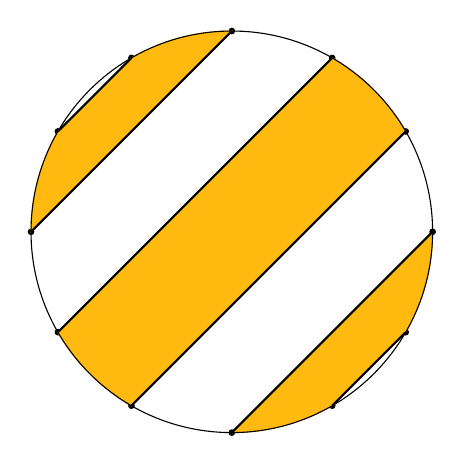
\begin{tikzpicture}[scale=0.85]
            \tcircle{0}{0}{3}{12}{0.05}{black};
            \draw[DarkGoldenrod1,fill=DarkGoldenrod1] (C9) arc [start angle=270, end angle=300, radius=3] -- (C11) arc [start angle=330, end angle=360, radius=3] -- (C9);
            \draw[thick,black] (C10) -- (C11) (C9) -- (C12);
            \draw[DarkGoldenrod1,fill=DarkGoldenrod1] (C7) arc [start angle=210, end angle=240, radius=3] --(C1) arc [start angle=30, end angle=60, radius=3] -- (C7);
            \draw[thick,black] (C7) -- (C2) (C1) -- (C8);
            \draw[DarkGoldenrod1,fill=DarkGoldenrod1] (C5) arc [start angle=150, end angle=180, radius=3] -- (C3) arc [start angle=90, end angle=120, radius=3] -- (C5);
            \draw[thick,black] (C6) -- (C3) (C5) -- (C4);
            \draw (O) circle (\radius);
          \end{tikzpicture}
        \end{minipage}\par%
        These are harder versions of the three circles in the Year 8 and below box, give those a try to warm up! As with those questions, each of these three pictures is a circle with twelve points spread equally around the circumference. The only other point used is the centre of the first circle (with the green shading). Find the proportion of each circle that is shaded.
      \iftoggle{SOLUTION}{%conditional output begin
      \begin{MySolutionBox}[skin=enhancedfirst]
        The Green One: We need to do a bit of dissecting here before we can move shaded areas into congruent unshaded areas. We draw in some radii and move the two segments downwards by one sector.\par
        \begin{minipage}[t]{0.25\linewidth}
          \strut\vspace*{-\baselineskip}\newline
        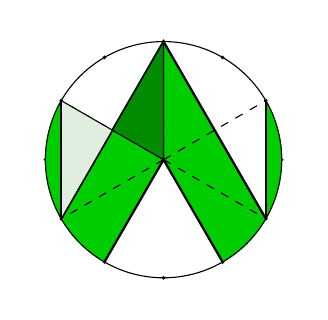
\begin{tikzpicture}[scale=0.5,background rectangle/.style={fill=white},show background rectangle]
            \tcircle{0}{0}{3}{12}{0.05}{black};
            \draw[Green3,fill=Green3] (C11) arc [start angle=-30, end angle=30, radius=3] --cycle;
            \draw[thick,black] (C11) -- (C1);
            \draw[Green3,fill=Green3] (C5) arc [start angle=150, end angle=210, radius=3] --cycle;
            \draw[thick,black] (C5) -- (C7);
            \draw[Green3,fill=Green3] (C7) -- (C3) -- (C11) arc [start angle=-30, end angle=-60, radius=3] -- (O) -- (C8) arc [start angle=240, end angle=210, radius=3] --cycle;
            \draw[thick,black] (C11) -- (C3) -- (C7) (C8) -- (O) -- (C10);
            \draw (O) circle (\radius);
            \draw[dashed] (O) -- (C1) (O) -- (C3) (O) -- (C5) (O) -- (C7) (O) -- (C11);
            \draw[dashed] (C11) -- (C1) (C5) -- (C7);
            \coordinate (M1) at ($(C3)!0.5!(C7)$);
            \draw[fill=Green4] (C3) -- (M1) -- (O) -- cycle;
            \draw[fill=Honeydew2] (M1) -- (C7) -- (C5) -- cycle;
          \end{tikzpicture}
        \end{minipage}%
        \begin{minipage}[t]{0.24\linewidth}
          \strut\vspace*{-\baselineskip}\newline
          \smallskip Next you can see that, by symmetry, the dark green shaded triangle is congruent to the pale grey-green triangle. So we can 'move' the green triangle into the 'empty' space. We can do exactly the same on the left-hand side of the circle.\par
        \end{minipage}%
        \begin{minipage}[t]{0.24\linewidth}
          \strut\vspace*{-\baselineskip}\newline
        \begin{tikzpicture}[scale=0.5,background rectangle/.style={fill=white},show background rectangle]
            \tcircle{0}{0}{3}{12}{0.05}{black};
            \draw[Green3,fill=Green3] (C11) arc [start angle=-30, end angle=30, radius=3] --cycle;
            \draw[Green3,fill=Green3] (C5) arc [start angle=150, end angle=210, radius=3] --cycle;
            \draw[Green3,fill=Green3] (C7) -- (M1) -- (C11) arc [start angle=-30, end angle=-60, radius=3] -- (O) -- (C8) arc [start angle=240, end angle=210, radius=3] --cycle;
            \draw[Green3,fill=Green3] (M1) -- (C7) -- (C5) -- cycle;
            \draw[Green3,fill=Green3] (C1) -- (O) -- (C11) -- cycle;
            \draw[thick,black] (O) -- (C1) (O) -- (C5) (C8) -- (O) -- (C10);
            \draw (O) circle (\radius);
            \draw[dashed] (O) -- (C7) (O) -- (C11) (C12) -- (C6);
          \end{tikzpicture}
        \end{minipage}%
        \begin{minipage}[t]{0.24\linewidth}
          \strut\vspace*{-\baselineskip}\newline
          You can see that six hour sectors are shaded, so we have shown that half of the circle was shaded green in the question.\par
        \end{minipage}\medskip\hrule\medskip
        The Blue One: Again, we need to try a bit of cutting. First notice that there is rotational symmetry. We can show that half of one of the blue bands is the same area as one 'hour' sector. Take a look at the dashed lines added to the middle puzzle above.\par
        \begin{minipage}[t]{0.33\linewidth}
          \strut\vspace*{-\baselineskip}\newline
          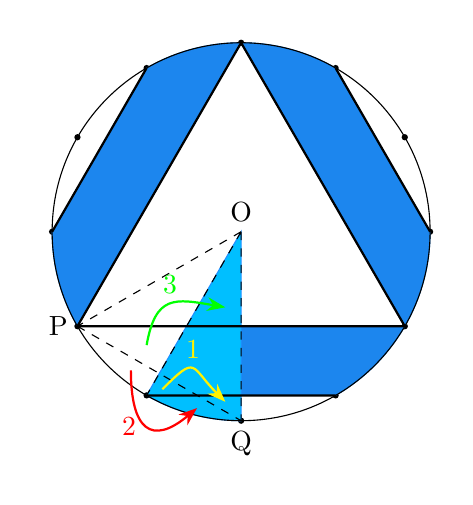
\begin{tikzpicture}[scale=0.8,background rectangle/.style={fill=white},show background rectangle]
            \tcircle{0}{0}{3}{12}{0.05}{black};
            \coordinate (M2) at ($(C7)!0.5!(C11)$);
            \coordinate (M3) at ($(C8)!0.5!(C10)$);
            \draw[DodgerBlue2,fill=DodgerBlue2] (C3) -- (C11) arc [start angle=-30, end angle=0, radius=3] -- (C2) arc [start angle=60, end angle=90, radius=3] -- (C7) arc [start angle=210, end angle=180, radius=3] -- (C4) arc [start angle=120, end angle=90, radius=3];
            \draw[DodgerBlue2,fill=DodgerBlue2] (C10) arc [start angle=300, end angle=330, radius=3] -- (M2) -- (M3) -- cycle;
            \draw[DodgerBlue1,fill=DeepSkyBlue1] (C8) arc [start angle=240, end angle=270, radius=3] -- (O) -- cycle;
            \draw[thick,black] (C11) -- (C3) -- (C7) --cycle;
            \draw[thick,black] (C12) -- (C2) (C4) -- (C6) (C8) -- (C10);
            \draw (O) circle (\radius);
            \draw[dashed] (O) -- (C8) (O) -- (C9) (C7) -- (C9) (O) -- (C7);
            \draw[-Stealth,thick,red] (-1.75,-2.2) to [out=-90,in=220,looseness=2.0] node[left] {\(2\)} (-0.7,-2.8);
            \draw[-Stealth,thick,yellow] (-1.25,-2.5) to [out=45, in=135,looseness=2] node[midway,yellow,above] {\(1\)} (-0.25,-2.7);
            \draw[-Stealth,thick,green] (-1.5,-1.8) to [out=80, in=170,looseness=1.5] node[midway,above,green] {\(3\)} (-0.25,-1.2);
            \node[above] at (O) {O};
            \node[left] at (C7) {P};
            \node[below] at (C9) {Q};
          \end{tikzpicture}
        \end{minipage}%
        \hfill
        \begin{minipage}[t]{0.6\linewidth}
          \strut\vspace*{-\baselineskip}\newline
          By symmetry, the small triangles marked by the yellow arrow \((1)\) are congruent, so we move the blue shaded area as indicated. Now we can move the half-segment as indicated by the red arrow \((2)\). Lastly, we can move the larger triangle as indicated by the green arrow \((3)\). The source triangle and destination triangle are congruent by symmetry in the equilateral triangle \(\bigtriangleup OPQ\). So now we have shown that the area of half of one of the original blue bands is the same as the area of one \SI{30}{\degree} sector. If we carry out the same procedure on the rest of diagram, we end up with six shaded sectors, we have shown that half the circle is shaded.\par
        \end{minipage}\medskip\hrule\medskip
      \end{MySolutionBox}
    \end{MyInnerBox}
    \newpage
    \begin{MyInnerBox}{Year 9 and above}
      \begin{MySolutionBox}[skin=enhancedlast]
        The Orange One: A bit harder, we have to do a little calculating for this one, unless you can find a better solution by dissection.\par
        \begin{minipage}[t]{0.4\textwidth}
          \strut\vspace*{-\baselineskip}\newline
          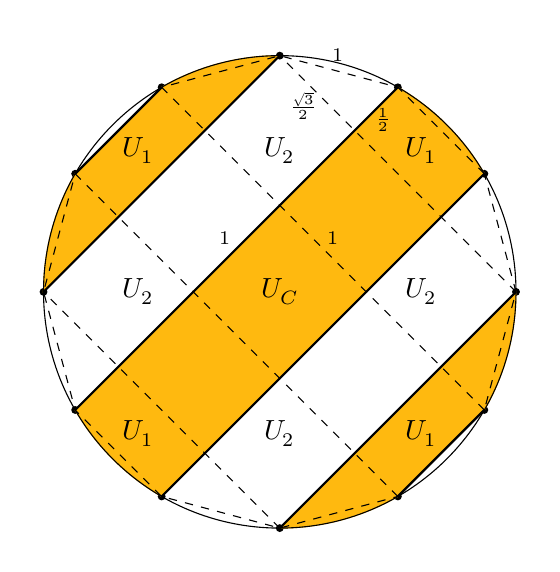
\begin{tikzpicture}[scale=1.0,background rectangle/.style={fill=white},show background rectangle]
            \tcircle{0}{0}{3}{12}{0.05}{black};
            \draw[DarkGoldenrod1,fill=DarkGoldenrod1] (C9) arc [start angle=270, end angle=300, radius=3] -- (C11) arc [start angle=330, end angle=360, radius=3] -- (C9);
            \draw[thick,black] (C10) -- (C11) (C9) -- (C12);
            \draw[DarkGoldenrod1,fill=DarkGoldenrod1] (C7) arc [start angle=210, end angle=240, radius=3] --(C1) arc [start angle=30, end angle=60, radius=3] -- (C7);
            \draw[thick,black] (C7) -- (C2) (C1) -- (C8);
            \draw[DarkGoldenrod1,fill=DarkGoldenrod1] (C5) arc [start angle=150, end angle=180, radius=3] -- (C3) arc [start angle=90, end angle=120, radius=3] -- (C5);
            \draw[thick,black] (C6) -- (C3) (C5) -- (C4);
            \draw (O) circle (\radius);
            \draw[dashed] (C1) \foreach \i in {2,...,12} { -- (C\i)} -- cycle;
            \draw[dashed] (C12) -- (C3) (C11) -- (C4) (C10) -- (C5) (C9) -- (C6);
            \node[above right=-0.1] at ($(C11)!0.5!(C4)$) {\(_{1}\)};
            \node[above left=-0.1] at ($(C2)!0.5!(C7)$) {\(_{1}\)};
            \node[above] at ($(C2)!0.5!(C3)$) {\(_{1}\)};
            \node[below left=-0.2] at ($(C3)!0.16!(C12)$) {\(_{\frac{\sqrt{3}}{2}}\)};
            \node[right] at ($(C2)!0.1!(C7)$) {\(_{\frac{1}{2}}\)};
            \node[] at (-1.8,1.8) {\(U_{1}\)};
            \node[] at (-1.8,-1.8) {\(U_{1}\)};
            \node[] at (1.8,-1.8) {\(U_{1}\)};
            \node[] at (1.8,1.8) {\(U_{1}\)};
            \node[] at (O) {\(U_{C}\)};
            \node[] at (-1.8,0) {\(U_{2}\)};
            \node[] at (0,-1.8) {\(U_{2}\)};
            \node[] at (1.8,0) {\(U_{2}\)};
            \node[] at (0,1.8) {\(U_{2}\)};
          \end{tikzpicture}
        \end{minipage}%
        \hfill
        \begin{minipage}[t]{0.55\linewidth}
          \strut\vspace*{-\baselineskip}\newline
          Notice that six of the small segments are shaded and six are not. So half of the twelve segments are shaded. Now examine the eight, congruent triangles. Four are shaded, four are not. Of the four rectangles surrounding the central \(1\) by \(1\) square, two are shaded, two are not.\par
          So far, of the shapes making up the whole circle, those not labelled U, \(50\%\) have been shaded.\par
          Now lets look at the remaining parts labelled U. (For unbalanced).\par
          If we say the length of each of the chords forming the segments is \(1\) then the sides of the triangle must be \(\frac{\sqrt{3}}{2}\) and \(\frac{1}{2}\) because each triangle has angles \(\SI{90}{\degree}\), \(\SI{30}{\degree}\) and \(\SI{60}{\degree}\). Why?\par
          Let's find the area of the unshaded 'U' areas.\par
          \(U_{2}\):  \(\qquad\qquad\: 4\times\left(\frac{\sqrt{3}}{2}\right)^{2} = 3\)\par
          Now let's find the area of the shaded 'U' areas.\par
          \(U_{1}+U_{c}\):  \(\qquad 4\times\left(1\times\frac{1}{2}\right) + 1\times 1 = 3\)\par
          So we have shown, once again, that the shaded area and the unshaded area is equal and so the circle is fifty percent orange.
        \end{minipage}
      \end{MySolutionBox}
    }{}%conditional output end
    \end{MyInnerBox}


  \end{MyOuterBox}

%%%%%%%%%%%%%%%%%%%%%%%%%%%%%%%%%%%%%%%%%%%%%%%%%%
\end{document}



